\section{INTRODUÇÃO}

Em condições de campo, as culturas estão sujeitas à perdas de área
foliar por diferentes causas, dentre elas o pastejo e a colheita
periódica das folhas, o ataque de insetos desfolhadores e de doenças
que causam sua queda ou necrose, as chuvas de granizo e a própria
senescência natural são as mais frequentes.  Uma desfolha
significativa reduz o potencial fotossintético e, dependendo da
intensidade e fase de crescimento da planta, ocasiona prejuízos à
produção \cite{Painter1981,Klubertanz1996}.  Algumas doenças e pragas,
fitotoxicidade de pesticidas ou adubos, granizo e certas injúrias
mecânicas são eventos comuns que causam desfolha em áreas de cultivo
de algodão e que podem prejudicar a produção e qualidade do produto
dessa cultura \cite{Silva2012a}.

\newpage
\section{MODELO}

A relação monótona não crescente entre produção e desfolha é a
informação preliminar considerada para elaborar um modelo. Dentre as
funções matemáticas que atendem à essa imposição, tem-se o modelo
potência, chamado de modelo Herschel-Bulkley por
\citeonline{Cheng1992}, como opção,
\begin{equation}
 f(x) = \theta_0-\theta_1 x^{\theta_2}, \qquad x\geq 0.
\end{equation}
A desfolha, $x$ (adimensional), assume valores entre 0 e 1.  A
produção normal, com unidade de medida representada por Y, prevista
sem haver desfolha é representada pelo parâmetro $\theta_0$ (Y), ou
seja, $f(0) = \theta_0$.  A redução na produção normal ao ocorrer uma
desfolha total é $\theta_1\geq 0$, ou seja, $f(0)-f(1) = \theta_1$.  O
parâmetro adimensional $\theta_2>0$ é um parâmetro de forma dessa
relação, que é côncava se $\theta_2>1$, convexa se $0<\theta_2<1$ e
linear se $\theta_2=1$. É conveniente reescrever o modelo considerando
a transformação $\theta_2 = \exp\{\theta_c\}$ uma vez que a função
exponencial é positiva e que isso não compromete a interpretação do
modelo em $\theta_2$ que é apenas um parâmetro de forma.  Dessa forma,
\begin{equation}\label{eq-modelo}
 f(x) = \theta_0-\theta_1 x^{\exp\{\theta_c\}}, \qquad x\geq 0,
\end{equation}
é uma função côncava para $\theta_c>0$, convexa para $\theta_c<0$ e
linear quando $\theta_c=0$ (Figura \ref{fig:herschel}).

\newpage
\section{MATERIAL E MÉTODOS}

\begin{figure}[!b]
\begin{center}
 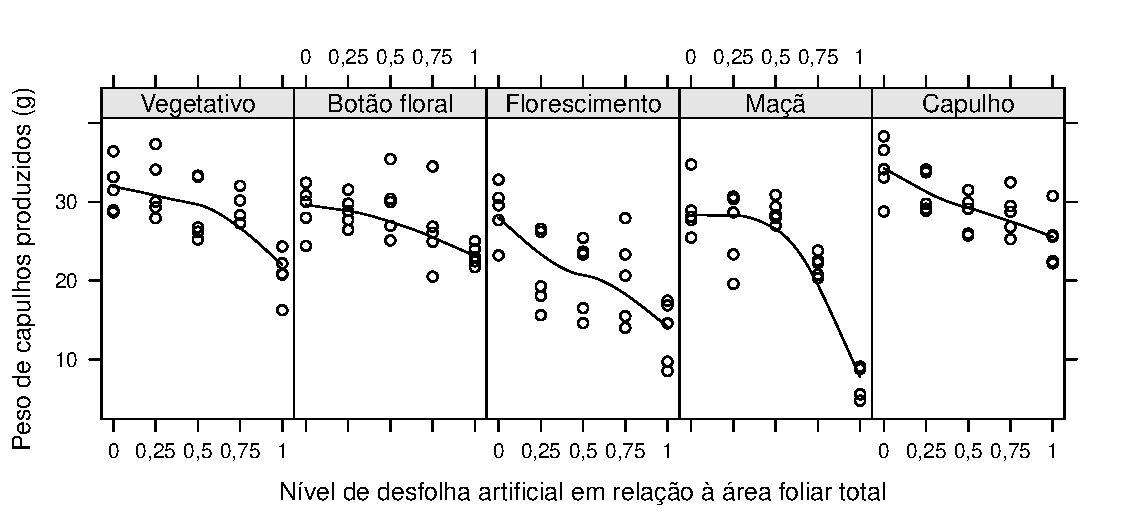
\includegraphics[width=\textwidth]{../figuras/previsu.pdf} 
\end{center}
\caption{Peso de capulhos produzidos (g) em cada estágio fenológico
  como função dos níveis de desfolha artificial. Curvas suaves entre
  os pontos representam as tendências centrais}\label{previsu}
\end{figure} 

Os dados considerados para ajuste do modelo são de um experimento, em
casa de vegetação, com a cultura do algodão (\emph{Gossypium
  hirsutum}). As unidades experimentais foram 2 plantas por vaso para
registro da produção total de pluma com caroço (g).  Os fatores
estudados foram o nível de desfolha artificial (0, 25, 50, 75 e
100\%), feita com tesoura em cada uma das folhas da planta conforme
tais níveis, combinados com o estágio fenológico no qual a desfolha
foi realizada (vegetativo, presença de botão floral, florescimento,
presença de maçã e presença de capulho). O delineamento completamente
ao acaso foi utilizado com cinco repetições, perfazendo $5\times
5\times 5 = 125$ unidades experimentais.  O experimento foi realizado
nas dependências da Universidade Federal de Grande Dourados no ano
agrícola de 2007. Mais informações disponíveis em
\citeonline{Silva2012a}.  Na Figura \ref{previsu} tem se o diagrama de
dispersão dos valores observados de peso de capulhos produzidos (g) em
cada estágio fenológico como função dos níveis de desfolha.

\newpage
\section{RESULTADOS E DISCUSSÃO}

Os ajustes dos modelos aos dados convergiram para os cinco estágios
fenológicos, considerando o máximo de 50 interações.  Valores iniciais
baseados na inspeção do diagrama de dispersão foram considerados
(Figura \ref{previsu}).  As estimativas dos parâmetros comuns,
$\theta_0$ e $\theta_1$, foram idênticas, em termos pontuais e
intervalares, nas duas parametrizações, como de fato devem ser pois
ambas parametrizações descrevem o mesmo modelo (Tabela
\ref{tb-estimic}). Percebeu-se um resultado alarmante para o estágio
de florescimento, no qual os intervalos de confiança para $\theta_0$ e
$\theta_1$ foram demasiado amplos, superando inclusive a amplitude
média de variação dos dados, de aproximadamente 5 g para cima e para
baixo, ao redor da curva de tendência.

\newpage
\section{CONCLUSÕES}

O propósito da reparametrização foi representar o nível de dano
econômico no modelo. As parametrizações foram comparadas com relação
aos métodos disponíveis para fazer inferência sobre o nível de dano
econômico. A inferência baseada em verossimilhança foi mais adequada
no sentido de auxiliar a seleção de modelos. Além do mais,
verificou-se que as medidas de curvatura e inspeção da matriz de
covariâncias das estimativas também são úteis no processo de seleção
de modelos. Nos estágios com pronunciada relação linear para
produção-desfolha, o modelo reparametrizado apresentou melhores
propriedades inferenciais.  O algodoeiro responde de forma
diferenciada à desfolha em cada estágio fenológico.

\newpage
\addcontentsline{toc}{section}{\hspace*{\distnumber}REFERÊNCIAS}
\begin{center}
\section*{REFERÊNCIAS} 
\end{center}
